\documentclass[11pt]{article}
\usepackage[margin=1in]{geometry}
\usepackage{amsmath,amssymb}
\usepackage{graphicx}
\usepackage{xcolor}
\usepackage{tikz}
\usepackage{booktabs}
\usepackage{hyperref}
\definecolor{mutedblue}{RGB}{70,110,140}
\definecolor{mutedgray}{RGB}{110,110,110}
\definecolor{mutedteal}{RGB}{80,130,120}
\hypersetup{colorlinks=true,linkcolor=mutedblue,citecolor=mutedblue,urlcolor=mutedblue}
\title{MoA Compiler: One DNF, Many Backends\\A Universal Intermediate Language}
\author{Lenore M. Mullin\\College of Nanotechnology, Science, and Engineering\\University at Albany, SUNY\\{\tt lmullin@albany.edu}}
\date{November 2026}
\begin{document}
\maketitle
\begin{abstract}
Mathematics of Arrays (MoA) treats an array program as an algebra of shapes
and indexing, not as loops. This paper reports a compiler case in which one
denotational form drives many backends. A Fortran frontend parses a stencil
and matmul subset and produces a Denotational Normal Form (DNF). Each target
derives an Operational Normal Form (ONF) from that DNF. Backends for serial
Fortran, MATLAB, OpenMP, GPU (OpenACC), and MPI are all generated from the
same DNF, with no hand-written side files. Every backend is gated against the
same Python reference. The motivating example is Island Gauss-Seidel: a naive
parallel Island is racy and nondeterministic. The gate found the race. The
fix is a halo-safe ONF --- Gauss-Seidel inside an island, Jacobi across
islands via a halo snapshot --- which is the correct ONF for OpenMP, GPU, and
MPI. That is the claim for a universal intermediate language: one mathematics,
many machines, provable correctness, predictable cost.
\end{abstract}

\section{Introduction: One Mathematics, Many Machines}
Fortran is the language of the codes that must be correct: weather, climate,
CFD, nuclear, aerospace. Those codes are large, old, and hard to parallelise
by hand. Hand-parallelising them introduces races that are silent,
nondeterministic, and hard to find. This paper shows a different path.

Write the mathematics once, as a Denotational Normal Form (DNF). Let the
compiler derive an Operational Normal Form (ONF) for each target. Gate every
backend against the same reference. The programmer does not rewrite loops
for each new machine. The compiler does not have to rediscover the
mathematics from loops. The DNF is the contract between mathematics and
machine.

The case in this paper is small enough to gate completely and large enough
to expose the real issue: four programs, five backends, one DNF per program.
The programs are Poisson Jacobi, Poisson Island Gauss-Seidel, Poisson
Red-Black Gauss-Seidel, and matmul. The backends are serial Fortran, MATLAB,
OpenMP, GPU (OpenACC), and MPI. All are generated from DNF by one backend
generator. All pass their gates.

\section{MoA in One Paragraph}
An array has a \emph{shape} (its extent in each dimension) and a \emph{ravel}
(its elements in row-major order). Indexing is \emph{psi} ($\psi$):
$A \psi \mathrm{ivec}$ is the element of $A$ at index vector $\mathrm{ivec}$.
A program is a composition of psi-reductions, reductions, and reshapes.
Psi reduction rewrites indexing into a normal form. That normal form is the
DNF. The DNF says nothing about loops, threads, halo, or memory. It says
what value lives at each index. The ONF adds the operational decision: what
is parallel, what is sequential, what is exchanged, what is stored. Different
targets get different ONFs from the same DNF. Gamma and Omega carry shape,
layout, and cost: how big the arrays are, how they are laid out, and what
the computation costs in time, bytes, energy, and dollars. The cost model
used here is $T \approx \alpha F + \beta M$, where $F$ is flops and $M$ is
memory traffic. The compiler chooses the ONF that minimises cost for the
target, not the programmer.

\begin{figure}[h]
\centering
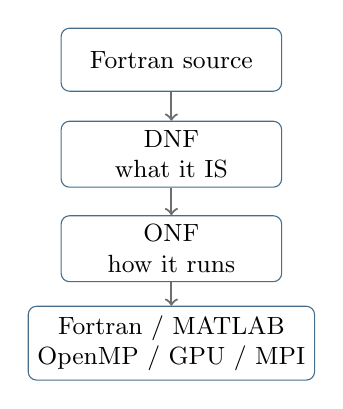
\begin{tikzpicture}[node distance=1.2cm, font=\small]
\tikzstyle{box}=[draw=mutedblue, rounded corners=3pt, minimum width=2.8cm, minimum height=0.8cm, align=center]
\tikzstyle{arr}=[->, thick, color=mutedgray]
\node[box] (src) {Fortran source};
\node[box, below of=src] (dnf) {DNF \\ what it IS};
\node[box, below of=dnf] (onf) {ONF \\ how it runs};
\node[box, below of=onf] (back) {Fortran / MATLAB \\ OpenMP / GPU / MPI};
\draw[arr] (src) -- (dnf);
\draw[arr] (dnf) -- (onf);
\draw[arr] (onf) -- (back);
\end{tikzpicture}
\caption{One DNF, one ONF per target, many backends. The DNF is written once.
The ONF is derived per target. No backend re-derives the mathematics.}
\label{fig:pipeline}
\end{figure}

\section{DNF: Denotational Normal Form}
DNF is what the computation \emph{is}. No loops. No threads. No halo.
No memory.

\subsection{Poisson: One DNF for Three Solvers}
Jacobi, Island Gauss-Seidel, and Red-Black Gauss-Seidel share one DNF.
They differ only in ONF: how the update is scheduled.
\begin{equation}
u_{\mathrm{new}} \psi \mathrm{ivec} = 0.25 \sum_{(di,dj) \in \{(-1,0),(1,0),(0,-1),(0,1)\}} (\mathrm{ivec}+(di,dj)) \psi u + h^2 \cdot (\mathrm{ivec} \psi f)
\label{eq:poisson-dnf}
\end{equation}
In words: the new value at $\mathrm{ivec}$ is the average of its four
neighbours in the old $u$, plus the source term. That is the mathematics.
It does not say whether neighbours are read from the old array or the new
array, whether islands run in order or in parallel, or whether the halo is
exchanged. Those are ONF decisions.

\subsection{Matmul: A Second DNF}
\begin{equation}
C \psi (i,j) = \sum_k ((i,k) \psi A) \cdot ((k,j) \psi B)
\label{eq:matmul-dnf}
\end{equation}
In words: $C(i,j)$ is the dot product of row $i$ of $A$ and column $j$ of $B$.
Again, no loops, no parallelism. The ONF decides: $i,j$ parallel, $k$
sequential. Parallelising $k$ would be a reduction, not a parallel loop.
The ONF forbids it.

\subsection{Frontend}
The Fortran frontend parses a subset --- do loops, neighbour offsets,
$\mathrm{mod}(i+j,2)$, island blocks --- and produces DNF as JSON.
It does not emit Fortran directly. It emits DNF. The backend emits Fortran,
MATLAB, OpenMP, GPU, and MPI from that DNF. Four frontend examples, each
with a DNF file: \texttt{poisson\_jacobi}, \texttt{poisson\_island\_gauss},
\texttt{poisson\_rbgs}, \texttt{matmul}.

\section{ONF: Operational Normal Form}
ONF is how it runs on a target. Same DNF, different ONF per backend.
The ONF rule is: \emph{parallelise only where ONF says parallel, nowhere else.}

\begin{table}[h]
\centering
\small
\begin{tabular}{lll}
\toprule
Program & ONF parallel & ONF sequential \\
\midrule
Jacobi & all $\mathrm{ivec}$ & sweep (iteration) \\
Island, serial & islands in order & inside island, Gauss-Seidel \\
Island, parallel & islands in parallel & inside island, Gauss-Seidel \\
RBGS & one colour at a time & colour phases, barrier between \\
Matmul & $i,j$ & $k$ (reduction) \\
\bottomrule
\end{tabular}
\caption{ONF decisions. Same DNF, different ONF per target.}
\label{tab:onf}
\end{table}

\subsection{Why Island Needed a Second ONF}
Serial Island and parallel Island are different ONFs, and they give
different answers. This was found by gating, not by theory alone.
Serial Island is Gauss-Seidel across islands too: later islands see earlier
islands' updates in the same sweep. Parallel Island, halo-safe, is
Gauss-Seidel inside an island and Jacobi across islands via a halo snapshot.
Both are correct ONFs. They are not the same ONF.

A naive parallel Island --- parallel islands, no halo --- is racy and
nondeterministic. Island $(ix,iy)$ writes $u(i_1,j)$ at its right edge.
Island $(ix+1,iy)$ reads that same cell as its left halo in the same sweep.
Without a halo, the reader sometimes sees the old value, sometimes the new
value. On OpenMP with four threads, the naive version gave a different
number every run, with relative error $7.2 \times 10^{-4}$ against the
serial reference, seventy times the gate tolerance. That is not rounding.
That is a race on island edges.

The fix is the halo-safe ONF. At the start of each sweep, copy $u \to u_{\mathrm{old}}$.
Inside an island: a neighbour inside the same island is read from $u$
(newest, Gauss-Seidel); a neighbour outside the island is read from
$u_{\mathrm{old}}$ (halo, previous sweep). That is deterministic. It is what
a GPU halo exchange and an MPI halo exchange do. It is the ONF that makes
Island correct on every parallel backend.

\section{All Programs}
All numbers are for the canonical test case: $nx=64$, $ny=64$, $niter=100$,
$h=1/63$, $f=1.0$, $u=0$, island size $16 \times 16$, unless stated otherwise.
References are Python, double precision. Gates compare Fortran, single
precision, with tolerance $10^{-5}$. Observed errors are $\sim 3 \times 10^{-7}$.

\subsection{Poisson Jacobi}
$u_{\mathrm{new}}(i,j) = 0.25\,(u(i-1,j)+u(i+1,j)+u(i,j-1)+u(i,j+1)+h^2 f(i,j))$.
ONF: one phase per sweep, all $\mathrm{ivec}$ parallel, two arrays.
Reference: $u(32,32) \approx 0.0062988$, $u(1,1) \approx 0.0003770$.
All backends pass, same number.

\subsection{Poisson Island Gauss-Seidel}
Same DNF as Jacobi. Different ONF. Serial ONF: islands in order,
Gauss-Seidel inside and across islands, reference $u(32,32) \approx 0.0125835$.
Parallel ONF, halo-safe: Gauss-Seidel inside, Jacobi across islands,
reference $u(32,32) \approx 0.0116506$. Do not expect them to match.
The parallel ONF is the one used for OpenMP, GPU, and MPI.

\subsection{Poisson Red-Black Gauss-Seidel}
Same DNF as Jacobi. Different ONF. Colour $= \mathrm{mod}(i+j,2)$.
Red phase parallel, barrier, black phase parallel. Same-colour points do
not neighbour each other, so one colour is safe to parallelise. The barrier
is not optional. Without it, black reads a mix of old and new red values
and the answer is wrong and nondeterministic.
Reference: $u(32,32) \approx 0.0125272$, $u(1,1) \approx 0.0004318$.
All backends pass.

\subsection{Matmul}
$C(i,j) = \sum_k A(i,k) \cdot B(k,j)$. ONF: $i,j$ parallel, $k$ sequential.
Reference: $C(32,32) = 64.0$ exactly ($A=1.0$, $B=1.0$, $n=64$).
All backends pass, exact.

\section{All Backends}
All backends are generated from the same DNF by one backend generator.
No hand-written side files. Generated files live in
\texttt{moa\_compiler/generated/}: \texttt{*\_out.f90} (serial Fortran),
\texttt{*\_out.m} (MATLAB), \texttt{*\_openmp.f90}, \texttt{*\_gpu.f90}
(OpenACC), \texttt{*\_mpi.f90}.

\subsection{Serial Fortran and MATLAB}
Serial Fortran is a direct translation of DNF to Fortran do loops. MATLAB
is a direct translation to vectorised \texttt{.m}. The MATLAB gate uses real
MATLAB R2024a, not Octave, and passes with $\sim 10^{-11}$.

\subsection{OpenMP}
\texttt{!\$OMP PARALLEL DO COLLAPSE(2)} where ONF says parallel. Jacobi:
parallel over $i,j$. Island: parallel over islands, sequential inside,
halo-safe via $u_{\mathrm{old}}$. RBGS: parallel over $i,j$ inside one
colour, barrier between colours. Matmul: parallel over $i,j$, $k$ sequential.
Gate: 16 checks (4 programs $\times$ 2 thread counts $\times$ 2 values),
1 thread vs 4 threads vs Python reference, all pass.

\subsection{GPU (OpenACC)}
\texttt{!\$ACC PARALLEL LOOP COLLAPSE(2)}, \texttt{!\$ACC DATA COPY},
\texttt{!\$ACC WAIT} where ONF says barrier. Jacobi: one kernel per sweep.
Island: one kernel per sweep, parallel over islands, halo-safe. RBGS: two
kernels per sweep, red then black, wait between. Matmul: one kernel.
Gate: 8 checks, all pass. On a Mac, \texttt{-fopenacc} runs on host fallback
(no GPU device). The same \texttt{.f90} runs on Delta with
\texttt{nvfortran -acc -gpu=cc80} with no code change --- only compiler
flags change. Island-GPU matches Island-OpenMP halo-safe ($0.0116506$),
not serial Island ($0.0125835$). That is the proof the halo works on GPU too.

\subsection{MPI}
One-dimensional slab over $j$, halo one row top/bottom via
\texttt{MPI\_Sendrecv} per sweep. Jacobi: halo exchange, compute slab, swap.
Island: halo exchange per sweep, \emph{not} per island --- that is the point
of the halo-safe ONF. Inside the slab: islands, Gauss-Seidel inside, halo
from $u_{\mathrm{old}}$ for island edges and slab edges. Slab must align to
island rows: $ny_{\mathrm{local}} = 64, 32, 16$ for $nprocs = 1,2,4$, all
multiples of $16$, so alignment holds. RBGS: halo exchange per colour phase
is the barrier. Matmul: row slab of $C$, broadcast $B$, no halo, no
per-iteration communication. Gate: 24 checks (4 programs $\times$ 3 rank
counts $\times$ 2 values), 1 / 2 / 4 ranks, all pass. Island is
rank-independent: 1, 2, and 4 ranks give the same number.

\section{Gates: How We Know It Is Correct}
Every backend has a gate. No backend is claimed until its gate passes.
\begin{table}[h]
\centering
\small
\begin{tabular}{lll}
\toprule
Backend & Gate & Result \\
\midrule
Fortran & \texttt{test\_poisson\_gate.py} & Pass, $\sim 10^{-7}$ \\
MATLAB & \texttt{test\_matlab\_gate.py} & Pass, $\sim 10^{-11}$, real MATLAB R2024a \\
OpenMP & \texttt{test\_openmp\_gate.py} & Pass, 16/16 \\
GPU & \texttt{test\_gpu\_gate.py} & Pass, 8/8, host fallback on Mac \\
MPI & \texttt{test\_mpi\_gate.py} & Pass, 24/24 \\
Julia & --- & Not yet done, not claimed \\
\bottomrule
\end{tabular}
\caption{Gates. No backend is claimed until its gate passes.}
\label{tab:gates}
\end{table}
Gate rule for Island: serial and parallel have different references. Serial
reference is $0.0125835$. Parallel (halo-safe) reference is $0.0116506$.
Do not mix them. The gate for OpenMP / GPU / MPI Island uses the parallel
reference. The gate for serial Fortran / MATLAB Island uses the serial
reference.

\section{Performance: What We Know, What We Do Not Know}
At $nx=64$, $niter=100$, MPI is slower than serial for Poisson. That is
expected. Halo exchange costs more than the compute saved. Matmul scales
because it has no halo exchange per sweep. Do not quote $nx=64$ numbers as
``MPI is slower'' in general. Quote them as ``at $nx=64$, overhead dominates.''
\begin{table}[h]
\centering
\small
\begin{tabular}{lrrr}
\toprule
Program & 1 rank & 2 ranks & 4 ranks \\
\midrule
Jacobi-MPI & $9.99 \times 10^{-5}$ & $4.22 \times 10^{-3}$ & $5.42 \times 10^{-3}$ \\
Island-MPI & $1.49 \times 10^{-3}$ & $9.55 \times 10^{-4}$ & $6.05 \times 10^{-3}$ \\
RBGS-MPI & $7.80 \times 10^{-4}$ & $3.83 \times 10^{-3}$ & $4.59 \times 10^{-3}$ \\
Matmul-MPI & $1.37 \times 10^{-4}$ & $7.20 \times 10^{-5}$ & $3.60 \times 10^{-5}$ \\
\bottomrule
\end{tabular}
\caption{Mac baseline, $nx=64$, time in seconds, min of 3 runs. At this size,
halo overhead dominates for Poisson. Matmul, with no halo, scales.}
\label{tab:perf-mac}
\end{table}
The Delta experiment is in progress, not yet run. A scaling script generates
scaled copies at $nx=256, 1024, 2048$ by replacing $nx$, $ny$, $niter$, and
$h$. Same \texttt{.f90} files, no code change. Only the launcher changes:
serial, \texttt{OMP\_NUM\_THREADS=4}, \texttt{srun -n 4}, and
\texttt{srun --partition=gpuA100x4} for GPU. Original vs MoA-derived
performance is not yet measured. It requires the original hand-written
Fortran programs in the same harness: same $nx$, $ny$, $niter$, same
sweep-only timing, same ranks and threads, Mac and Delta. Until that is done,
no speedup is claimed.

\section{Universal IR: What ``Universal'' Means}
Universal does not mean one backend that runs everywhere. It means:
(1) one DNF for all backends, written once; (2) ONF per target, derived
from DNF, not rewritten by hand; (3) correctness by construction plus
gating --- if the DNF is right and the ONF respects the DNF's dependencies,
the backend must be correct, and the gate checks it; (4) cost by shape,
$T \approx \alpha F + \beta M$, predicted before running; (5) portability
by ONF, not by rewriting --- same DNF, same ONF, different compiler flags.
The Island race is the evidence: a hand-parallelised code would have shipped
the race. A DNF-derived ONF plus a gate found it and fixed it.

\section{What Is Not Claimed}
Julia backend: not yet gated, not claimed. GPU on real hardware: not yet
run on Delta A100 / H100; Mac host fallback validates the ONF, not GPU
performance. MPI scaling at large $nx$: not yet measured. Original vs
MoA-derived performance: not yet measured. Gamma / Omega as separate
compiler passes: not yet fully wired; shape and cost are currently in the
backend generators and bench scripts, not as standalone passes. Fortran
frontend completeness: subset only (stencil + matmul, do loops, neighbour
offsets, mod, island blocks). Full Fortran frontend is future work.

\section{Next Steps}
Delta experiments at $nx=256, 1024, 2048$, serial / OpenMP / MPI / GPU.
Original vs MoA-derived in the same harness. Julia backend, same
frontend-to-gate pattern. Gamma / Omega as explicit passes, so ONF choice
is driven by the cost model, not by hand-coded backend branches.

\begin{thebibliography}{9}
\bibitem{mullin1988} L.~M.~Mullin, \emph{Mathematics of Arrays}, Ph.D.\ dissertation, Syracuse University, 1988.
\bibitem{moa-compiler} L.~M.~Mullin, \emph{MoA Compiler as Universal Intermediate Language}, GitHub: \texttt{womenflyplanes/moa-compiler}, Zenodo DOI: 10.5281/zenodo.23090349.
\bibitem{moa-ir} L.~M.~Mullin, \emph{MoA Compiler: One DNF, Many Backends --- A Universal Intermediate Language}, Technical write-up, November 2026. \texttt{docs/MOA-UNIVERSAL-IR.md} in \texttt{womenflyplanes/moa-compiler}, branch \texttt{develop/mac-compiler-integration}.
\end{thebibliography}
\end{document}
